\documentclass[aspectratio=169]{beamer}

\usepackage{global-macros}
\usepackage{graphicx}
\graphicspath{{../fig}}
\usepackage{algpseudocode, algorithm}
\usepackage{biblatex}

\vfuzz=30pt


\addbibresource{../bib/bibliography.bib}

\title{NPIV estimation through functional SGD}
\author{Student: Caio Lins
        \\ Advisor: Yuri Saporito
}
\institute{EMAp -- FGV}
\date{\today}

\titlegraphic{
    
\includegraphics[width=3cm]{logo.png}
}

\AtBeginSection[]
{%
  \begin{frame}
    \frametitle{Summary}
    \tableofcontents[currentsection]
  \end{frame}
}

\addtobeamertemplate{navigation symbols}{}{%
    \usebeamerfont{footline}%
    \usebeamercolor[fg]{footline}%
    \hspace{1em}%
    \insertframenumber/\inserttotalframenumber
}

\newcommand{\boldf}{\boldsymbol{f}}

\newcommand{\hstar}{h^{ \star }}
\newcommand{\risk}{\mathcal{R}}
\newcommand{\loss}{\ell}
\renewcommand{\hat}{\widehat}
\newcommand{\iid}{\overset{\mathrm{iid}}{\sim}}
\DeclareMathOperator{\diam}{diam}
\newcommand{\data}{\mathcal{D}}
\newcommand{\dataproj}{\mathcal{D}_{ \mathrm{proj} }}


\begin{document}

    \frame{\titlepage}

    \section{NPIV estimation}

    \begin{frame}{Instrumental Variables}
        \begin{itemize}
            \item<1-> Consider a generic regression problem:
                \begin{equation*}
                    Y = \hstar ( X ) + \varepsilon
                ,\end{equation*}
                where $ \mean [ \varepsilon ] = 0 $ and we wish to estimate $ h^{ \star } $.

                \item<2-> What happens if $ \varepsilon \not\kern-1pt\indep X $? More specifically, if $ \mean [ \varepsilon \mid X ] \neq 0 $?
                \item<3-> Minimizing $ \mse ( h ) = \mean [ ( Y - h ( X ) )^2 ] $ over $ h $ gives biased results:
                \uncover<4->{
                    \begin{equation*}
                        \argmin_{ W = h ( X ) \text{ for some } h } \mean [ ( Y - W )^2 ]
                        = \mean [ Y \mid X ]
                        = \hstar ( X ) + \underbrace{\mean [ \varepsilon \mid X ]}_{\neq 0}
                    .\end{equation*}
                }
                \item<5-> We end up estimating $ \hstar ( X ) + \mean [ \varepsilon \mid X ] $.
                    Other problems may occur.
        \end{itemize}
    \end{frame}

    \begin{frame}{Instrumental Variables}
        \begin{itemize}
            \item<1-> Suppose we have access to a variable $ Z $ such that
                \begin{enumerate}
                    \item<2-> $ p_{ X\mid Z } ( x \mid z ) $ is not constant in $ z $, that is, $ Z $ influences $ X $;
                    \item<3-> $ \varepsilon $ is uncorrelated with $ Z $, that is, $ \mean [ \varepsilon \mid Z ] = 0 $.
                \end{enumerate}
                \uncover<5->{$ Z $ is called an \emph{instrumental variable}.}
                \item<6-> How does it help us?
        \end{itemize}
    \end{frame}

    \begin{frame}{Instrumental Variables}
       \begin{itemize}
           \item<1->  Structural equation:
               \begin{equation*}
                   Y = \hstar ( X ) + \varepsilon
               ,\end{equation*}
               where $ \mean [ \varepsilon \mid Z ] = 0 $.
           \item<2-> Consider minimizing $ \risk ( h ) = \mean \left[ \left( \mean [ Y - h ( X ) \mid Z ] \right)^2 \right] $ over $ h $.
            \item<3-> Compare:
                \begin{equation*}
                    {\color{red}
                        \mse ( h ) = \mean [ ( Y - h ( X ) )^2 ]
                    }
                    \quad \text{v.s.} \quad
                    {\color{blue}
                        \risk ( h ) = \mean \left[ \left( \mean [ Y - h ( X ) \mid Z ] \right)^2 \right] 
                    }
                .\end{equation*}
       \end{itemize} 
    \end{frame}

    \begin{frame}{Instrumental Variables}
        \begin{itemize}
            \item<1-> Since
                \begin{equation*}
                    \mean [ Y \mid Z ]
                    = \mean [ \hstar ( X ) + \varepsilon \mid Z ]
                    = \mean [ \hstar ( X ) \mid X ] + \cancelto{0}{\mean [ \varepsilon \mid Z ]}
                    = \mean [ \hstar ( X ) \mid Z ]
                ,\end{equation*}
                \uncover<2->{
                    We have
                    \begin{align*}
                        \risk ( h )
                        &= \mean \left[
                            \left(
                                \mean \left[
                                    Y - h ( X ) \mid Z
                                \right]
                            \right)^2
                        \right] \\
                        &= \mean \left[
                            \left(
                                \mean \left[
                                    ( \hstar - h ) ( X )
                                    \mid Z
                                \right]
                            \right)^2
                        \right]
                    .\end{align*}
                }
                \item<3-> $ \risk ( h ) = 0 \iff \mean \left[ \left( \hstar - h \right) ( X ) \mid Z \right] = 0 \iff \mean [ \hstar ( X ) \mid Z ] = \mean [ h ( X ) \mid Z ] $.
        \end{itemize}
    \end{frame}

    \begin{frame}{Example}
        \begin{equation*}
            \underbrace{\text{Grades}}_{Y} = \hstar \bigl( \underbrace{ \text{Attends tutoring sessions?} }_{X} \bigr) + \varepsilon
        .\end{equation*}
        \begin{itemize}
            \item<2-> Natural ability is a confounding variable: maybe only people who struggle a lot go to tutoring sessions.
            \item<3-> $ Z = \text{Lives close to school?} $
                \begin{enumerate}
                    \item<4-> $ Z \not\kern-1pt\indep X $,
                    \item<4-> $ \varepsilon \indep $ Z $ $.
                \end{enumerate}
        \end{itemize}
    \end{frame}

    \begin{frame}{NPIV estimation}
        \begin{itemize}
            \item<1-> Stands for ``Nonparametric Instrumental Variable estimation''.
            \item<2-> No assumptions on some parametric form for $ \hstar $.
        \end{itemize}
    \end{frame}

    \section{Our approach}

    % Stochastic gradient computation
    % Pseudo algorithm

    \begin{frame}{Problem Formulation}
        \begin{itemize}
            \item<1-> We have
                \begin{equation}
                    \label{eq: structure}
                    Y = \hstar ( X ) + \varepsilon   
                ,\end{equation}
                 where $ \mean [ \varepsilon \mid Z ] = 0 $, and want to estimate $ \hstar $.
             \item<2-> Let $ \meanop [ h ] = \mean [ h ( X ) \mid Z = \cdot ] $, that is
                 \begin{equation*}
                     \meanop [ h ] ( Z ) = \mean [ h ( X ) \mid Z ]
                 .\end{equation*}
             \item<3-> Let $ r_{ 0 } ( Z ) = \mean [ Y \mid Z ] $.
                 Then (\ref{eq: structure}) is equivalent to:
                 \begin{equation*}
                     \mean [ Y \mid Z ] = \mean [ \hstar ( X ) \mid Z ] \iff r_{ 0 } = \meanop [ \hstar ]
                 .\end{equation*}
            \item<4-> We wish to ``invert'' $ \meanop $.
            \item<4-> Risk measure:
                \begin{equation*}
                    \risk ( h ) = \mean \left[ \frac{ 1 }{ 2 } \left( \mean \left[ Y - h ( X ) \mid Z \right] \right)^2 \right] = \mean \left[ \frac{ 1 }{ 2 } \left( r_{ 0 } ( Z ) - \mathcal{T} [ h ] ( Z ) \right)^2 \right]
                .\end{equation*}
        \end{itemize}
    \end{frame}
    \begin{frame}{Problem Formulation}
        \begin{itemize}
            \item<1-> Our risk measure:
                \begin{align*}
                    \risk ( h )
                    &= \frac{ 1 }{ 2 } \mean \left[
                        \left(
                            \mean \left[
                                Y - h ( X ) \mid Z
                            \right]
                        \right)^2
                    \right] \\
                    &= \frac{ 1 }{ 2 } \mean \left[
                        \left(
                            r_{ 0 } ( Z ) - \meanop [ h ] ( Z )
                        \right)^2
                    \right] \\
                    &= \frac{ 1 }{ 2 } \mean \left[
                        ( r_{ 0 }  - \meanop [ h ] ) ( Z )^2
                    \right]
                .\end{align*}
        \end{itemize}
    \end{frame}

    \begin{frame}{Stochastic Gradients}
        \begin{itemize}
            \item<1-> We showed that $ \nabla \risk ( h ) = \meanop^{ * } [ \meanop [ h ] - r_{ 0 } ] $, where
                \begin{equation*}
                    \meanop^{ * } [ f ] ( X ) = \mean [ f ( Z ) \mid X ]
                .\end{equation*}
            \item<2-> Immediate idea:
                \begin{equation*}
                    \begin{cases}
                        h_{ 0 } \equiv 0, \\
                        h_{ t } \leftarrow h_{ t-1 } - \alpha_{ t } \nabla \risk ( h_{ t-1 } ) \quad \text{for} $ t \geq 1 $.
                    \end{cases}
                \end{equation*}
                \item<3-> There are problems\dots
        \end{itemize}
    \end{frame}

    \begin{frame}{Stochastic Gradients}
        \begin{itemize}
            \item<1-> Another idea: notice that
                \begin{align*}
                    \meanop^{ * } [ f ] ( x )
                    &= \mean \left[ f ( Z ) \mid X = x \right] \\
                    &= \int_{ \mathcal{Z} } f ( z ) p ( z \mid x ) \ \mathrm{d}z \\
                    &= \int_{ \mathcal{Z} } f ( z ) \frac{ p ( x, z ) }{ p ( x ) p ( z ) } p ( z ) \ \mathrm{d} z \\
                    &= \mean \left[ f ( Z ) \Phi ( x, Z ) \right]
                ,\end{align*}
                where $ \Phi ( x, z ) = \frac{ p ( x, z ) }{ p ( x ) p ( z ) } $.
            \item<2-> In the spirit of SGD, $ f ( Z ) \Phi ( x, Z ) $ is a stochastic estimate for $ \meanop^{ * } [ f ] ( x ) $.
        \end{itemize}
    \end{frame}
    \begin{frame}{Stochastic Gradients}
        \begin{itemize}
            \item<1-> Substitute $ \nabla \risk ( h ) = \meanop^{ * } [ \meanop [ h ] - r_{ 0 } ] $ for
                \begin{equation*}
                    \hat{ \Phi } ( \cdot, Z ) \left(
                        \hat{ \meanop } [ h ] ( Z ) - \hat{ r_{ 0 } } ( Z )
                    \right)
                .\end{equation*}
            \item<2-> New algorithm:
                \begin{equation*}
                    \begin{cases}
                        h_{ 0 } \equiv 0, \\
                        h_{ t } \leftarrow h_{ t-1 } - \alpha_{ t } \hat{ \Phi } ( \cdot, Z_{ t } ) \left(
                            \hat{ \meanop } [ h ] ( Z_{ t } ) - \hat{ r_{ 0 } } ( Z_{ t } )
                        \right) \quad \text{for} $ t \geq 1 $.
                    \end{cases}
                \end{equation*}
                \item<3-> We chose to use RKHS (kernel) methods for computing $ \hat{ \Phi }, \hat{ \meanop } $ and $ \hat{ r_{ 0 } } $.
        \end{itemize}
    \end{frame}

    \section{Where we are at}

    \begin{frame}{Prototype}
        Prototype gave reasonable results
        \begin{figure}[htb]
            \begin{center}
                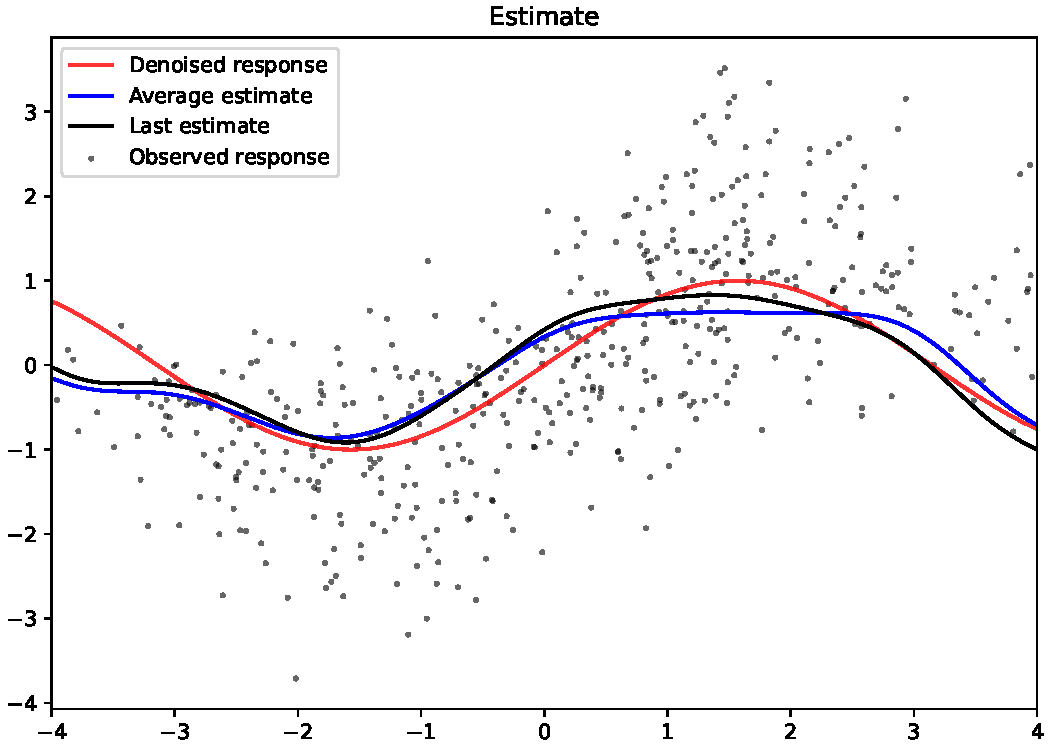
\includegraphics[width=.5\textwidth]{estimate.pdf}
                \caption{In red we have $ \hstar = \sin $, in black we have $ h_{ N } $ and in blue, $ \frac{ 1 }{ N } \sum_{ t=1 }^{ N } h_{ N } $.}
                \label{fig: prototype}
            \end{center}
        \end{figure}
    \end{frame}

    \begin{frame}{Theoretical properties}
        \begin{itemize}
            \item<1-> Still working on convergence guarantees.
            \item<2-> This is helping us find better ways to estimate $ \Phi $ and $ \mathcal{T} $ (mainly RKHS methods).
        \end{itemize}
    \end{frame}

    \section{Next steps}

    \begin{frame}{Next steps}
        \begin{itemize}
            \item<1-> Finalize convergence guarantees.
            \item<2-> Implement modifications which the theory points to.
            \item<3-> Benchmark against current methods.
        \end{itemize}
    \end{frame}

    \begin{frame}
        \frametitle{References}
        \nocite{*}
        \printbibliography
    \end{frame}

    \begin{frame}
        \centering Thank You!
    \end{frame}

\end{document}
